\documentclass[4pt,a4paper]{article}
\usepackage[blocks]{authblk}
\usepackage[utf8]{inputenc}
\usepackage[english]{babel}
\usepackage{algorithm}
\usepackage{textcomp}
\usepackage{fontenc}
\usepackage{tipa}
\usepackage{multicol}
\usepackage{lscape}
\usepackage{color}
\usepackage{graphicx}
\usepackage{enumerate}
%\usepackage{epsfig}
%\usepackage{epstopdf}
\usepackage{amsmath}
\usepackage{framed}


\begin{document}
\author{David Przybilla\footnote{dav.alejandro@gmail.com},\hspace{3 mm}Sibel Ciddi\footnote{sciddi@coli.uni-sb.de},\hspace{3 mm}Noushin Fadaie\footnote{nfadaei@coli.uni-sb.de},\hspace{3 mm}Moinuddin Haque\footnote{moinuddinmushirul@gmail.com}}
%\affil[]{\textit{sciddi@coli.uni-sb.de, nfadaei@coli.uni-sb.de, dav.alejandro@gmail.com, moinuddinmushirul@gmail.com}}
\affil{Universit\"at des Saarlandes\\ \small Computational Linguistics \& Phonetics,\\Saarbr\"ucken, Germany}
\title{Fast Search for Named Entity Recognition\\ \large Summer 2012: Basic Algorithms for Computational Linguistics}
\maketitle

\begin{abstract}
In this paper, we present three different approaches based on Approximate Dictionary Matching Algorithm that uses similarity measures for the retrieval of Named Entities. For the evaluation, we extracted PERSON Named Entity types from the CoNLL-2003 Shared Task Corpus Data. In order to determine the fastest search approach, for the results, we compare CoNLL data the average processing times outputted by these different dictionary implementations.\\\textbf{keywords}: Information Extraction, dictionary search, similarity measures, simString, Named Entities, NEs, NER.
\end{abstract}
%newpage

\section{Introduction}
\label{sec:intro}

Due to the problematic identification of Named Entities, collecting Named Entities in the field of Information Extraction and Natural Language Processing has been a popular task during the past years. There have been more than several methods that deal with this specific task; both from a statistical point of view, and rule-based method point of view, for extraction of Name Entities(NE) from raw text. On this paper, we present \texttt{NERSimString}, which is a Java library, based on an approximate dictionary matching algorithm\cite{Okazaki:Coling2010}\footnote{http://www.chokkan.org/software/simstring}that uses various similarity measures. This algorithm targets the retrieval of strings faster for Named Entity Recognition systems. The main idea behind the \texttt{NERSimString} is that it creates a library for storing Name Entity dictionaries, and at the same time provides a quick Named Entity annotation tool for the given named entity dictionaries generated by the system.\\

In most NER systems, creating  and storing NE dictionaries can raise some problems. Even in most state-of-the-art NER systems, generated NE dictionaries, to be used as fixed-lists later, impose the following issues that still remain challenging to resolve:
\begin{itemize}
	\item Even in a restricted domain, the number of Named Entities in a dictionary can be overwhelming.
	\item Considering the size of a corpus, when the fixed-dictionaries are given, the final goal of finding all the NEs contained in a corpus can still be a hard task.  
	\item Even in semi-supervised methods that are trained to recognize the NEs require fast searching tools; because the training requires searching and finding the location of a given set of NE that is located in a corpus.
\end{itemize}

Therefore, in order to make the annotation task of Named Entities a tractable problem, a method that looks for words quickly in a huge dictionary becomes mandatory. The \texttt{NERSimString} algorithm precisely targets to handle this specific problem and aims to achieve an accurate and fast searching method.

%\newpage

\section{The SimString Method}
\label{sec:simString}
For more straightforward and simpler NER tasks with a narrower focus, exact dictionary look-up methods can be used as well. However, besides non-user generated data, the SimString method targets the user generated data \emph{(i.e., social network corpus)} as well. Because user-generated data can have many variations, including potentially misspelled words, while dealing with user-generated data, \texttt{NERSimString} offers fast, approximate string retrieval. In these terms, it provides a quick way to make the search on the cost of space.\\
%\subsection*{What does NERSimString offer?}

In the \texttt{NERSimString} algorithm, \texttt{NerSimString} dictionary is  created from a list of items made of one Named Entity--\emph{which can be multi-word}--per line. Fast search queries can be requested via this dictionary. On this paper, for the purpose of comparing different dictionary set-ups; we adopted three different low-level implementations\footnote{The implementation source code is available at: https://github.com/dav009/NERSimString}:
\begin{enumerate}
 	\item \textbf{SuffixTree Implementation:} A dictionary based on a suffix tree to hold in memory
 	\item \textbf{Naive-HashTable Implementation:} A dictionary based on hash tables to hold in memory
 	\item \textbf{MemoryMapped Hashtable Implementation:} A dictionary based on hash maps, that is meant for large amounts of data. In order to avoid being completely loaded into memory, it is dynamically stored in the disk.\end{enumerate}
%\subsection*{What kind of similarities?}

In order to provide approximate string retrieval, the following similarity measures have been used:\\
\begin{enumerate}[i.]
			\item Jaccard
			\item Dice
			\item Cosine
\end{enumerate}
%\subsection*{Why is it fast?}
With these settings, \texttt{NERSimString} works fast by creating an inverted list of the size of n-grams. Based on one of the given similarity measures and a specific threshold, it measures how many n-grams at a certain length are the most likely to match the given NE query. This enables the system to discard as many alternatives as possible, which then makes the fast search possible. Thus, given these settings, the SimString model can be used both for the annotation of Named Entities and for the extension of current NER systems that are trained to predict Named Entities.
%newpage

\section{The SimString Algorithm}
\label{sec:algorithm}
\begin{landscape}

\begin{figure}[h!]
  \caption{Overview of the SimString Algorithm}
  \centering
  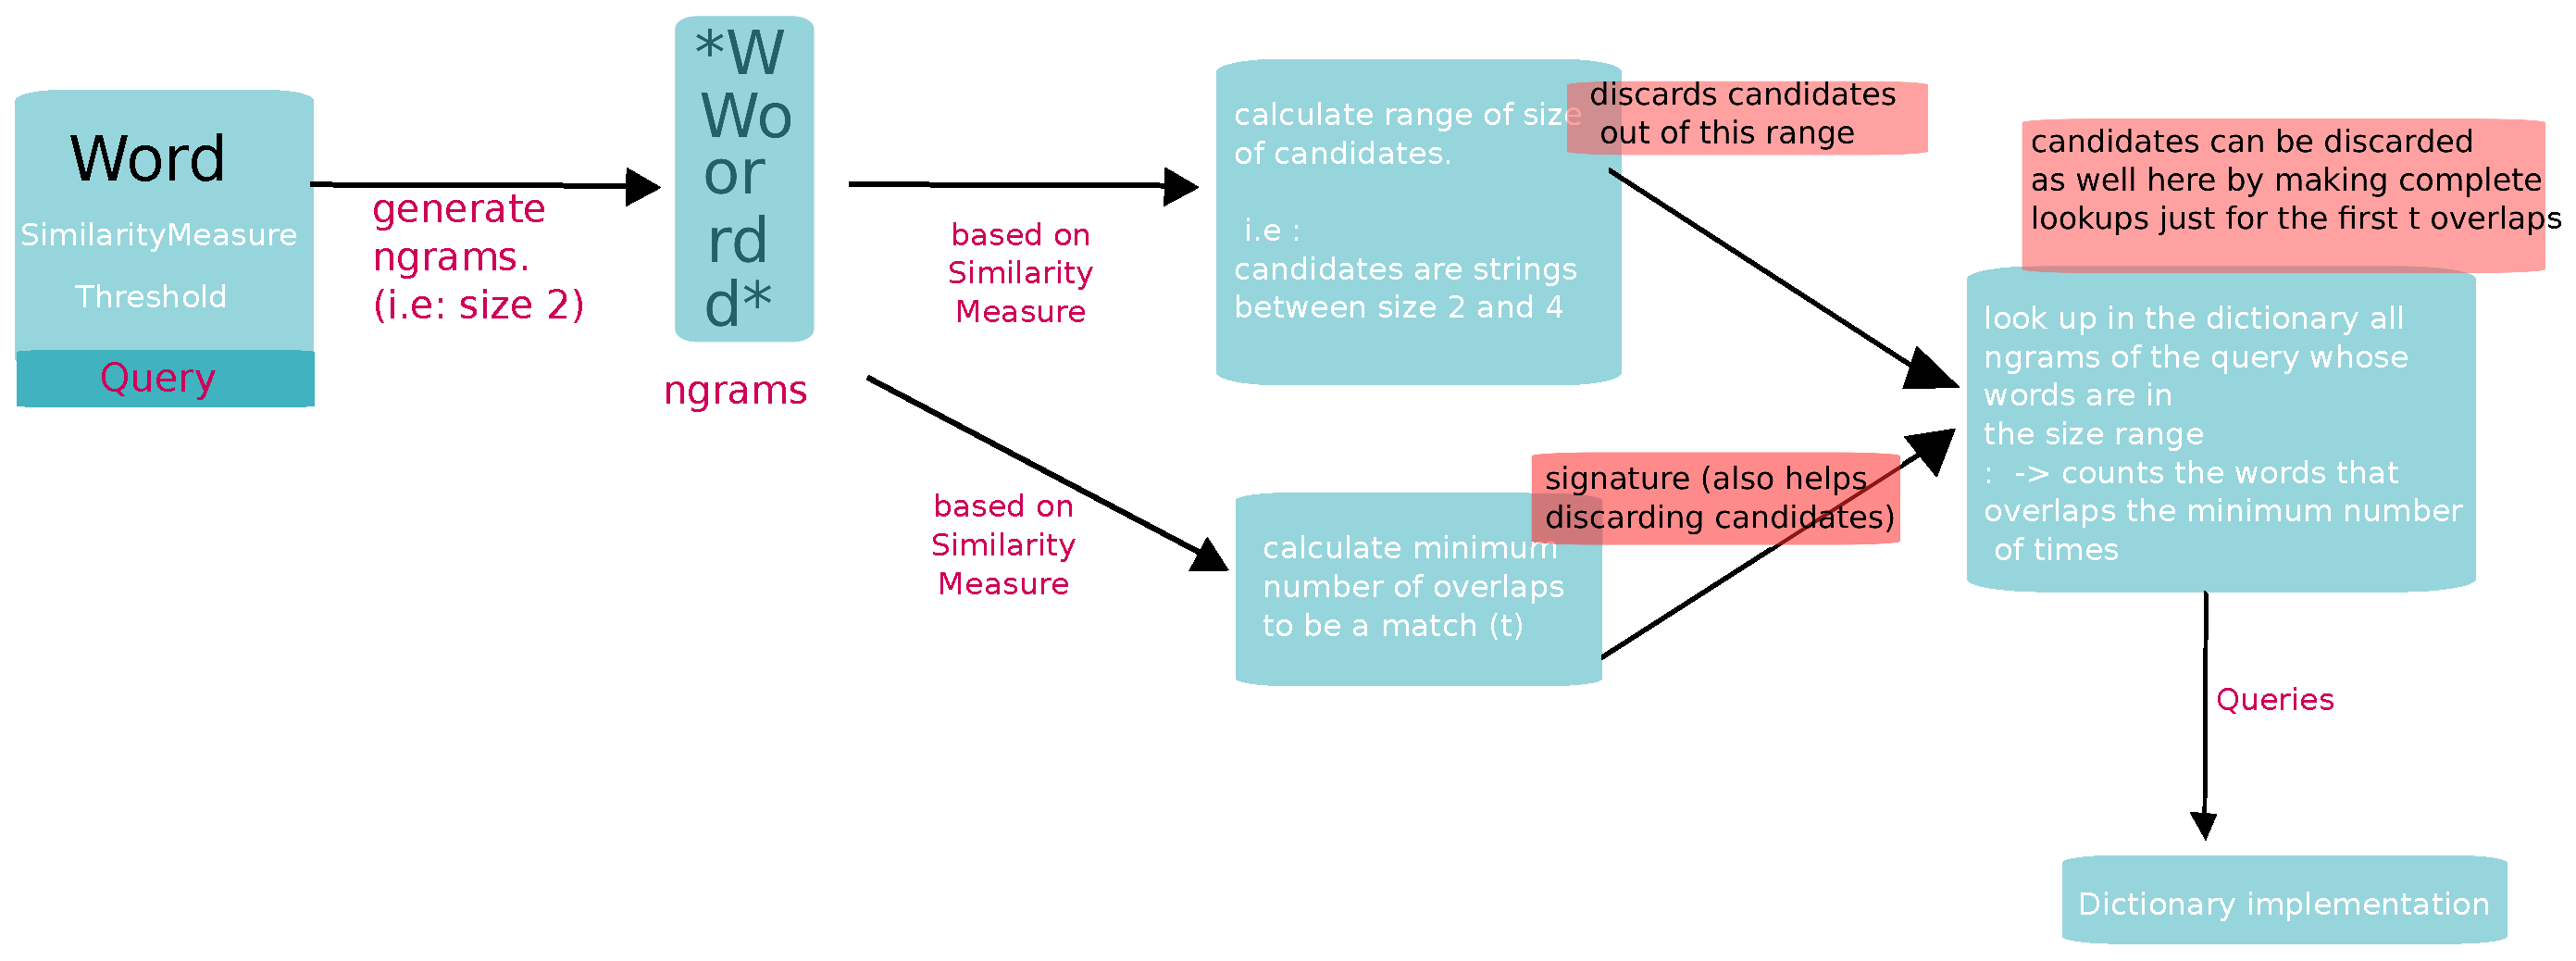
\includegraphics[scale=0.45]{graphics/simStringAlgorithm}
  \label{fig:simStringAlgorithm}  
\end{figure}

\end{landscape}


%\newpage

\section{Implementation}
\label{sec:implementation}
The concept behind the implementation was to make a highly object oriented framework
so that the different parts could be replaced by new ones transparently and thus allowing
for further experimentation and expansion of the tool.
The chosen language for the implementation was Java, since Java is a popular programming language
it opens up the possibility of using the tool with many other packages or even as a webservice
for more sophisticated applications.

\subsection{Packages}

This is a description of the most important  packages and classes related to the implementation:


\subsubsection*{IO}
The classes in this package have the responsability of dealing with
the input/output files.\\
The class DictionaryReader.java is incharged of reading a raw dictionary file (one entry per line).

\subsubsection*{Measures}
This package is composed of all classes relating the different similarity measures.
The SimString algorithm is independant of the chosen similarity, for doing this
an interface called $Similarity$ exists within the package, in order to extend
the system to provide new similarities measures this interface has to be implemented.\\
\\
Aditionally this package has a class name MeasureFactory, which is incharged of constructing
similarities's objects.

\begin{figure}[h!]
  \caption{Class Diagram with respect to Similarity classes}
  \centering
    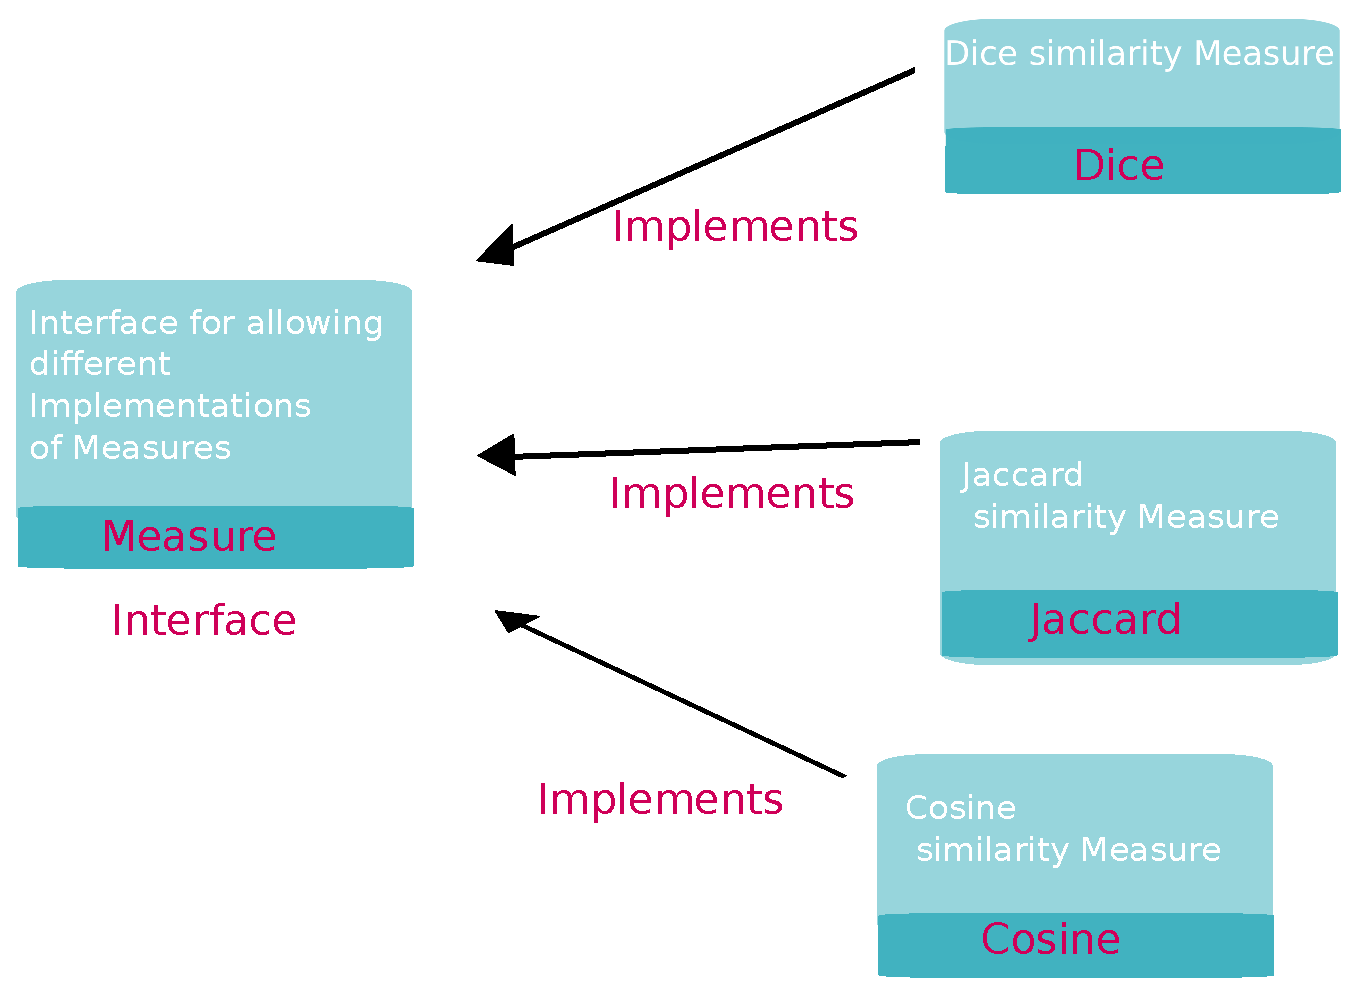
\includegraphics[scale=0.45]{graphics/similarities}
   \label{fig:similarityClasses}  
\end{figure}


\subsubsection*{Dictionary}
This package contains all the classes which have a responsability related to dictionaries.\\
\\
Among the most important ones are $LowLevelDictionaryImplementation$ this is an interface
which allows the tool to implement differnt kinds of Dictionary Implementations, for example
one dictionary can be represented either as a hashtable or as suffixtree, while those
data structures are different by implementing $LowLevelDictionaryImplementation$ they become
transparent to the simString algorithm.\\
\\
Additionally this package contains all the classes related to the different offered implementations
of dictionaries.




\subsubsection*{SimString}
This package contains the class $SimString$ which given a dictionary,a similarity configuration  and a query
is able to search in the dictionary and retrieve all the similar NE given the value of the parameters.


\subsubsection*{Util}
This package is composed of different classes with different responsabilities.
The $NGram$ class is incharged of splitting words into ngrams and dealing with any specific functionality related to ngrams.

\subsubsection*{Examples}
This package contains classes (each one is an example) for the potential users.

\subsubsection*{Test}
This package contains classes which allow team to asses the time performance of the tool and make comparisons among the different implementations.


\subsection{Dictionary Implementations}


As an addition to the simstring algorithm, the team introduced different ways to implement
the underlying data structure representing the ngram-inverted index.\\
\\
There are two types of data structures alternatives: mapped and not mapped.
Not mapped data structures are traditional data structures, that is, structures that are kept entirely on memory while the program is running. \\
As opposed to this type  there are mapped data structures which are data structures saved in the hard disk
and as data from it is needed small chunks of the datastructure are loaded into memory.\\
\\
The memory mapped data structures are ideally for cases when the number of data being stored is very high and having the whole datastructure in memory at once is not feasible.
However memory mapped data structures come with a cost: $Memory$.\\
Since memory mapped data structure implementations want to be as fast as traditional data structures, they have to be stored in memory in a way they can be queried quickly.\\
The only way to assure this is by having a fixed number of bits used per data field in the mapped data structure,this means, that no matter the size of the data, a slot in this structures will always have a fix size, this means using extra memory.


\begin{figure}[h!]
  \caption{The Dictionary Implementations}
  \centering
    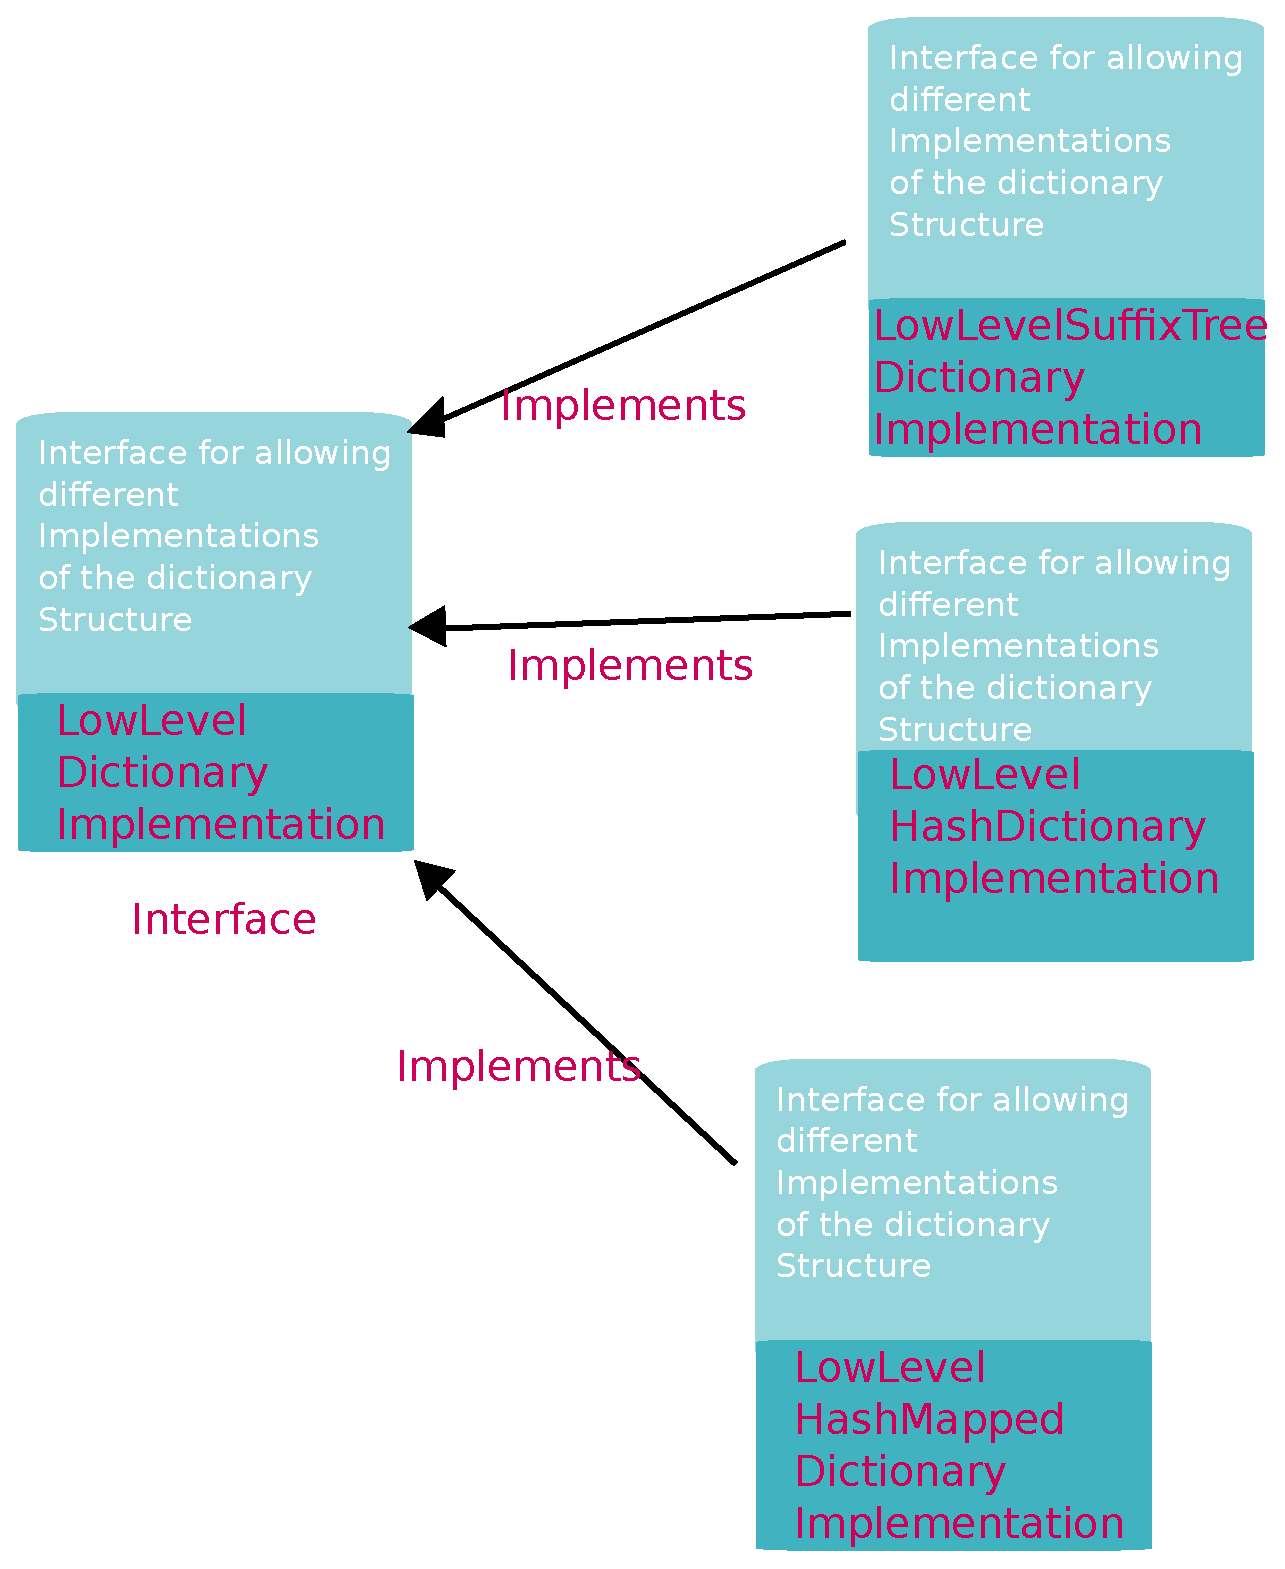
\includegraphics[scale=0.45]{graphics/dictionaryImplementations}
   \label{fig:dictionaryClasses}  
\end{figure}



\subsubsection{SuffixTree}  

This is an implementation of the inverted index of ngrams by using suffixTrees.\\
The keys in this case are strings of the shape: $ngram$-$sizeOfString$, the values are Priority Queues with the id's of dictionary entries which size is $sizeOfString$ and contains the given  $ngram$.

\subsubsection{Naive-HashTable}
 This is an implementation of the inverted index of ngrams by using Java HashMaps.\\
The keys in this case are strings of the shape: $ngram$-$sizeOfString$, the values are Priority Queues with the id's of dictionary entries which size is $sizeOfString$ and contains the given  $ngram$.
  
\subsubsection{MemoryMapped Hashtable}
 This is an implementation of the inverted index of ngrams by using memory mapped Hashtables.\\
It allows to save the generated dictionary in a file and to load it for later use.

\begin{figure}[h!]
  \caption{Comparison between Mapped Datastructures and not mapped}
  \centering
    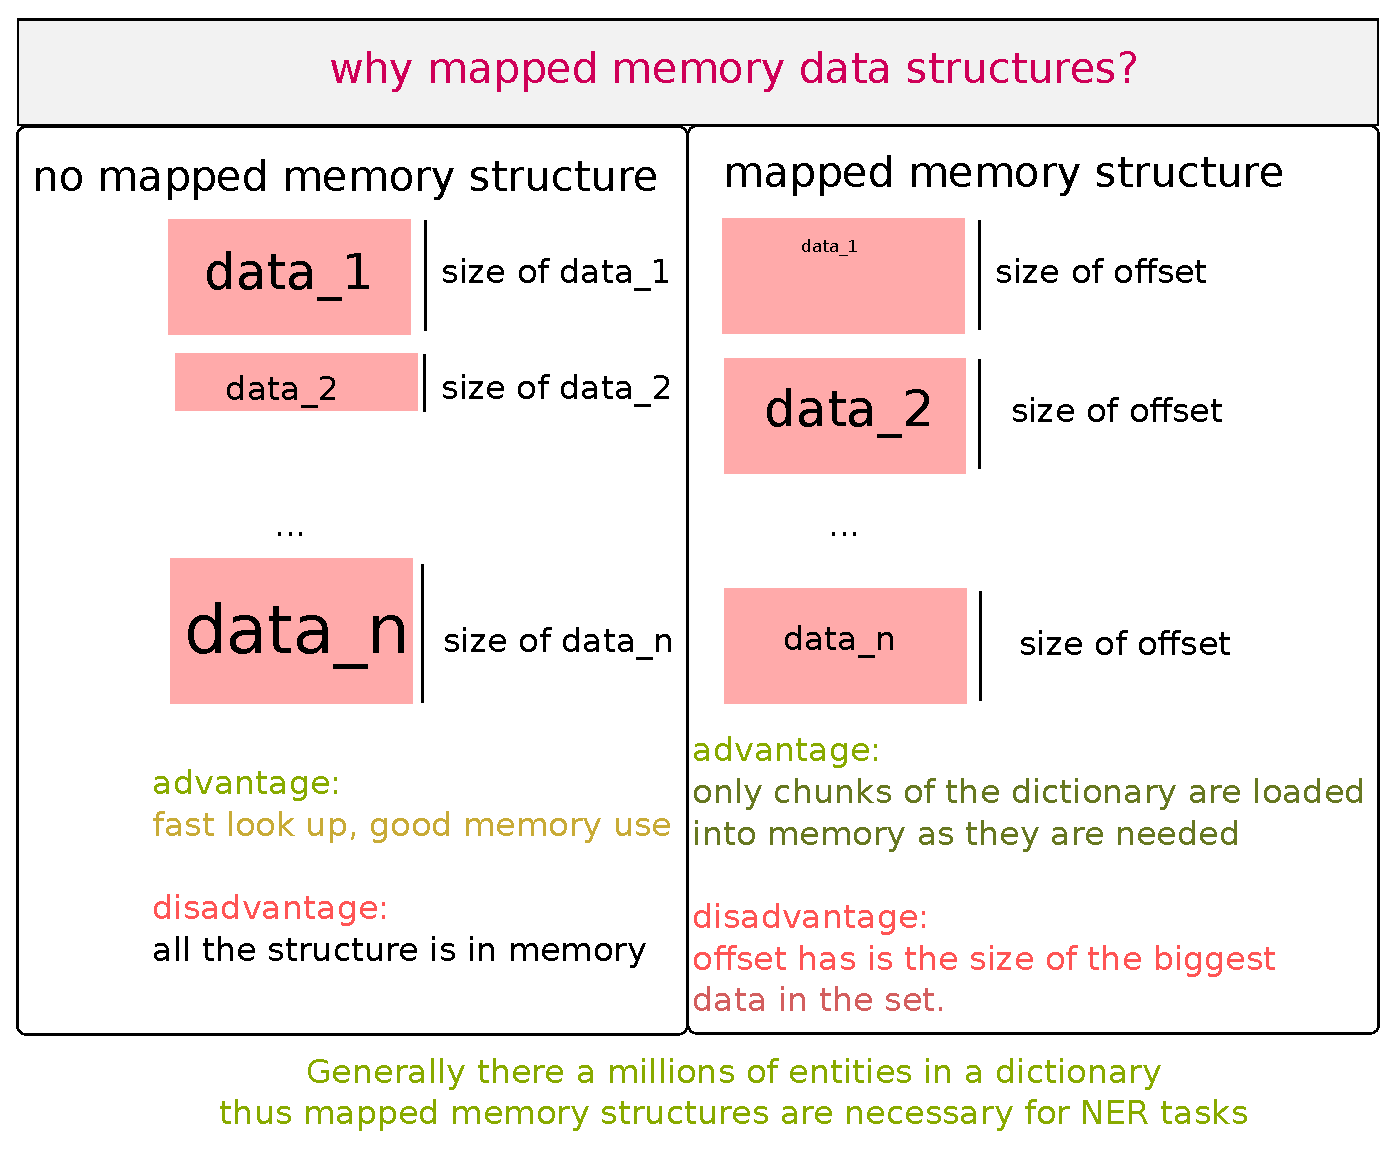
\includegraphics[scale=0.5]{graphics/memoryMappedVsNonMemoryMapped}
   \label{fig:mappedDataStructures}  
\end{figure}


  

%\newpage

\section{Evaluation and Results}
\label{sec:results}
\texttt{NERSimString} algorithm with three different dictionary implementations were evaluated by using the CoNLL-2003 Shared Task Data Corpus\footnote{Data files available at: http://www.clips.ua.ac.be/conll2003/ner/} \footnote{English data set request from: http://trec.nist.gov/data/reuters/reuters.html}. We compared the dictionary implementation models against the original SimString algorithm implementation as the baseline. The evaluation of these different implementations measured the average processing time\//\textit{per second} of the dictionaries by considering the given \texttt{n-gram} sizes and different similarity \texttt{thresholds}.

We evaluated these dictionaries on two different CoNLL data settings, only for PER (\textit{person\_NE}) Named Entity type:
\begin{enumerate}[i.]
	\item First, we tested the dictionaries by taking 200 \textbf{random} search strings per method.
	\item Second, we tested the dictionaries by taking the first 200 words from the CoNLL corpus.
\end{enumerate}

The following tables show the results for the average processing times returned by each of the dictionary implementations:

\begin{center}

\begin{table}[H]
\scalebox{0.9}{
  \begin{tabular}{| l | c | c | c | c | r| }
    
    \hline
    \textbf{ } & \textbf{SuffixTree} & \textbf{HashTable} & \textbf{Mapped HashTable} & \textbf{SimString}\\ \hline
    \texttt{Threshold} & 0.2 & 0.2 & 0.2 & 0.2   \\ \hline
    \texttt{N-Gram:3-Avg.Time} & 0.26034846156 & 0.1600577245 & 0.38093002297 & 0.1198204536   \\ \hline
    \texttt{N-Gram:5-Avg.Time} & 0.13545810821 & 0.1907321242 & 0.13516753774 & -   \\ \hline
    \texttt{N-Gram:8-Avg.Time} & 0.18630211667 & 0.1774560892 & 0.19634142339 & -   \\ \hline

    \hline
  \end{tabular}
  }
  \caption{Average Look-up Time Results Based on 200 Random Strings}
  \end{table}
  
\end{center}

\begin{center}

\begin{table}[H]
\scalebox{0.9}{
  \begin{tabular}{| l | c | c | c | c | r| }
    
    \hline
    \textbf{ } & \textbf{SuffixTree} & \textbf{HashTable} & \textbf{Mapped HashTable} & \textbf{SimString}\\ \hline
    \texttt{Threshold} & 0.8 & 0.8 & 0.8 & 0.8   \\ \hline
    \texttt{N-Gram:3-Avg.Time} &   0.317907188  & 0.611821308 & 1.132227919 & 2.774974599   \\ \hline
    \texttt{N-Gram:5-Avg.Time} &   0.448093155  & 0.599589026 & 1.480562861 & -   \\ \hline
    \texttt{N-Gram:8-Avg.Time} &   1.003509663  & 2.200090178 & 1.927359551 & -   \\ \hline
    
    \hline
  \end{tabular}
  }
  \caption{Average Look-up Time Results Based on First 200 Strings on CoNLL Data}
  \end{table}  
\end{center}

These results show that the \texttt{SuffixTree} and the regular\textit{(naive)} \texttt{HashTable} Dictionary implementation outputs were relatively close to the original \texttt{SimString} algorithm implementation. The \texttt{Mapped HashTable} Dictionary handled the data input efficiently as well, however due to the construction of memory mapped structure, the average look-up times resulted in more time than the other two dictionary implementations.



	
	
%\newpage

\section{Conclusion and Future Work}
\label{sec:conclusion}
On this paper, we presented different implementations of the proposed \texttt{SimString} algorithm. We found out that the implementation of \texttt{SimString} is easily extensible for different approaches. Some of the implementations are more useful for other tasks like fast look-up, and for Named Entity Recognition, which is one of the problematic areas in natural language processing and information extraction. We found out that the \texttt{SuffixTree} and \texttt{HashTable} dictionaries returned the relatively similar and fast average look-up times for potential Named Entity candidates. With the different implementations of the inverted dictionary indexes we have presented, we can conclude that they provide different applications, and they were useful in evaluating the performance of the implementation for comparison purposes.\\

Some of the research areas that can be looked further in detail, for example, would be building a \texttt{bootstrapper} for learning Named Entities based on the different implementations of the \texttt{SimString} algorithm, such as the \texttt{NERSimString} dictionaries we presented on this paper. Adding extra similarity measures alternatives for testing and training might also help finding out the best approach for that kind of applications.\\

More sophisticated NER systems can benefit from the \texttt{SimString} implementations by further expanding it with \textit{signature information} which can be extracted from the dictionaries. This info could include anything from finding the \textit{upper and lower boundaries} of NE candidates to applying Noun-Phrase Chunking on the NE Candidates returned from the dictionaries.\\

Besides the potential \textit{bootstrapping} oriented implementation or more sophisticated NER system; adding more support for \texttt{Memory-Mapped HashTable} dictionaries might also be useful for other applications. For the basic NER system, it is expected to see that the \texttt{Mapped HashTable} Dictionaries outputted the slowest search look-up times for Named Entity candidates. However, this does not mean that the \texttt{Mapped HashTable} dictionaries are not a good candidate implementation for other look-up applications, that require a lot of data to be held on the memory. For example, for spell-checker application dictionaries, especially for languages with a large lexicon \textit{(e.g., highly-inflected languages)}, the use of \texttt{Mapped HashTable} dictionary implementation would be very beneficial.\\

Another functionality could be easily added in order to improve this algorithm when searching for Name Entities,
that is for example saving extra information, (a small simstring dictionary for example) with signatures for allowing a better candidate selection with dealing with this task.
When it comes to this task, the simstring structure could also be extended for holding more than one value per key,this  allowing a single dictionary to hold different kinds of name entities.\\

As a final note, for this project, we would like note that researching about different implementation techniques and learning about the differences in application to search look-up was an enjoyable learning task. Because information extracting and search techniques is one of the most challenging--and at the same time rewarding tasks in NLP, we plan on continuing on working on the mentioned research areas for future research.
%\newpage
\bibliographystyle{plain}
\bibliography{simString}
\end{document}